% Need to explain NCBI, BLAST

There are some terms that will be used later in the report that should
be clarified here, so as to avoid confusion.
The aim of the project is to creating a teaching tool for PCR, or
Polymerase Chain Reactions.
This is the process of amplifying a specified sequence of DNA thousands to
millions of times.
It should be explained that DNA sequences are made up of two strands,
comprised of bases of the nucleotides Adenine, Thymine, Guanine and
Cytosine, represented by the letters \verb£a£, \verb£t£, \verb£g£, and
\verb£c£ respectively.
Base pairing is when one base bonds with its complement on the other
strand.
The bases \verb£a£ and \verb£t£ complement each other, and bases
\verb£g£ and \verb£c£ complement each other.

Primers, used to select the sequence for PCR in a given selection of
DNA, are shorter fragments of DNA, usually between 20 and 30 bases in
length.
For use in PCR, a primer must be chosen from the ``left'' of one
strand (this is the forward primer) and the ``right'' of the other
(this is the reverse primer), and these must obey a number of rules,
which are the focus of the teaching tool:
\begin{itemize}
\item Neither primer should self-anneal. 
  This means that if the primer were to fold over
  in such a way that that more than 3 bases in a row on one side
  complemented the bases on the opposite side, this primer would pair 
  with itself and become useless for the purposes of PCR.
\item The melting temperature of each primer, calculated in degrees
  Celsius using a simple mathematical formula involving the frequency
  of \verb£a£s, \verb£t£s, \verb£g£s and \verb£c£s, should be between
  50 and 65\degree C, and within 2-3\degree C of each other.
\item The forward primer should be unique within the first strand, and
  not appear in the second, complementary strand. Likewise, the
  reverse primer should be unique within the second strand and should
  not appear in the first.
\item The percentage of \verb£g£s and \verb£c£s within each primer
  should be between 40\% and 60\%.
\item The length of each primer should be between 20 and 30 bases.
\item The same base should not be repeated several times in a row in
  either primer.
\item The last base of each primer should be either a \verb£g£ or a
  \verb£c£.
\item The primers should not anneal to each other. 
  This means that if the primers were put side by side, at no point of
  overlap should more than 3 bases in a row complement the overlapping
  primer’s base.
\end{itemize}

It should be noted that many of these rules are not precise, and do
not involve rigid limits for success or failure.
In fact, these ``rules'' more closely resemble rough guides.
Obviously, the nature of programming does not lend itself to ``rough
guides'', and so we followed advice from Pamela Scott and Nicola
Veitch on how best to structure these tests to effectively represent
the imprecision of their boundaries.

%----------------------------YO ROSS START HERE---------------------------

\begin{figure}[!t]
  \begin{center}
    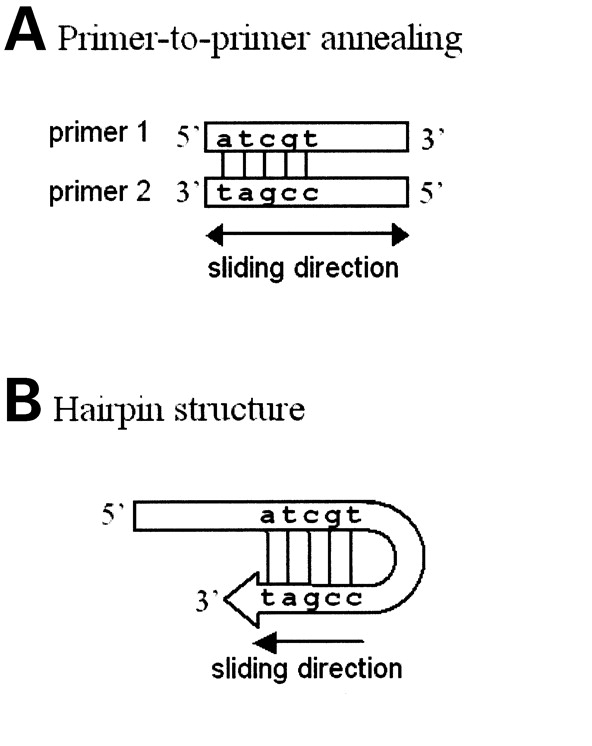
\includegraphics[width=0.75\textwidth]{./images/other/annealing.jpg}
    \caption{
      \label{fig:other:anneal}
      Annealing	
    }
  \end{center}
\end{figure}








%--------------------------------------------------------------------------

Two external services that are integral to the successful use of the system
are the National Center for Biotechnology Information (NCBI) \cite{ncbi},
and the use of a Basic Local Alignment Search Tool. NCBI is, for the purposes
of this exercise, a vast database of DNA sequences and related information,
from which the user can obtain a sequence on which to perform PCR (though this
can also be obtained from other sources). At the end of the exercise, the
user is encouraged to use the BLAST functionality on the NCBI website to ensure
that their primer is specific to their intended PCR target.

It should also be explained that we developed the teaching tool
in Java, using Netbeans, a free IDE primarily designed to be used with
Java, and developing the user interface with Swing, the primary Java 6
GUI framework and that we stored all project-related files in a
version-controlled repository hosted by GitHub.

